\documentclass[a4paper,12pt]{article}
\usepackage{polski}
\usepackage[utf8]{inputenc}
\usepackage[left = 3cm, right = 3cm, top = 2cm, bottom = 2cm]{geometry}
\usepackage{enumerate}
\usepackage{amssymb}		% pakiet do symboli
\usepackage{mathtools}		% pakiet do matmy (rozszerza amsmath)
\usepackage{enumitem}		% punktowanie (a), (b), ...
\usepackage{nopageno}		% brak numerow stron
\usepackage{graphicx}		% wstawianie obrazkow
\usepackage{float}			% wstawianie obrazkow w dowolnym miejscu
\usepackage{caption}
\usepackage{esdiff}         % pochodne \diff{}{}
\usepackage{listings}
\usepackage{xcolor}
\usepackage{adjustbox}

% nowe komendy dla wygodniejszego pisania :)

\newcommand{\floor}[1]{\left\lfloor #1 \right\rfloor}	% podłoga
\newcommand{\ceil}[1]{\left\lceil #1 \right\rceil}		% sufit
\newcommand{\fractional}[1]{\left\{ #1 \right\}}		% część ułamkowa {x}
\newcommand{\abs}[1]{\left| #1 \right|}					% wartosc bezwzgledna / moc
\newcommand{\set}[1]{\left \{ #1 \right \}}				% zbiór elementów {a,b,c}
\newcommand{\pair}[1]{\left( #1 \right)}				% para elementów (a,b)
\newcommand{\Mod}[1]{\ \mathrm{mod\ #1}}				% lekko zmodyfikowane modulo
\newcommand{\comp}[1]{\overline{ #1 }} 					% dopełnienie zbioru 
\newcommand{\annihilator}{\mathbf{E}}					% operator E
\newcommand{\seqAnnihilator}[1]{\annihilator \left\langle #1 \right\rangle} % E(a_n)
\newcommand{\sequence}[1]{\left\langle #1 \right\rangle} % <a_n>
\DeclareMathOperator{\lcm}{lcm}							% obsługa lcm w mathmode

% styl do kodu
\lstdefinestyle{code}{%
basicstyle=\ttfamily\small,
commentstyle=\color{green!60!black},
keywordstyle=\color{magenta},
stringstyle=\color{blue!50!red},
showstringspaces=false,
numbers=left,
numberstyle=\footnotesize\color{gray},
numbersep=10pt,
tabsize=4,
rulecolor=\color{red},
breaklines=true
}

\newcommand{\code}[1]{\lstinline[style=code]{#1}} % kod inline

\begin{document}
\noindent \textbf{Matematyka dyskretna L, Lista 9 - Tomasz Woszczyński}\newline

\noindent \newline \textbf{Zadanie 1} \newline
Przedstaw algorytm, służący do sprawdzania, czy dany graf jest dwudzielny,
korzystający z przeglądania grafu metodą w głąb (DFS). Złożoność Twojego 
algorytmu powinna być $O(m+n)$. \\

\noindent Aby dowiedzieć się, czy graf jest dwudzielny, możemy wykorzystać 
kolorowanie wierzchołków. Jeżeli graf da się pokolorować na dwa kolory, to
graf jest dwudzielny.

\begin{lstlisting}[style=code, language=python]
visited = [False, ..., False] # length n
color   = [False, ..., False] # length n; assume False is red
                              # and True is green

# execute DFS with colouring from any vertex v, but make sure
# that visited[v] is True and color[v] is False (red)
def is_bipartite(G, v, visited, color):
    for u in neighbours[v]:
        # if vertex u has not been visited, mark it as 
        # visited, color it according to v's color, then
        # execute DFS from vertex u to go deeper and deeper
        # until we check all neighbours of u
        if not visited[u]:
            visited[u] = True
            color[u] = not color[v]

            # run DFS on currently visited vertex
            if not DFS(G, u, visited, color)
                return False
        
        # if vertex u has been visited and v's and its
        # colors are the same, then G is not bipartite
        elif color[v] == color[u]:
            return False

    return True
\end{lstlisting}

\noindent Jako że korzystamy z lekko zmodyfikowanego DFS i przechodzimy wszystkie
wierzchołki i krawędzie, to złożoność tego algorytmu to $O(m + n)$, gdzie $n$ to
liczba wierzchołków, a $m$ to liczba krawędzi. W zależności od gęstości krawędzi
w grafie $G$, wartość $O(m)$ może być pomiędzy $O(1)$ i $O(n^2)$.

\newpage
\noindent \textbf{Zadanie 2} \newline
Niech $t_i$ oznacza liczbę wierzchołków stopnia $i$ w drzewie. Wyprowadź dokładny
wzór na $t_1$, liczbę liści w dowolnym drzewie. Dlaczego ta liczba niezależy od $t_2$? \\

\noindent Wiemy, że liczbę krawędzi dla $n$-wierzchołkowego drzewa można policzyć
na kilka sposobów, nas szczególnie interesują dwa poniższe:
\begin{enumerate}
    \item z lematu o uściskach dłoni:
    \[ 
        2 \abs{E} = \sum\limits_{i = 1}^{n} \deg(v_i) = \sum\limits_{i = 1}^{n} (i \cdot t_i)
        \Longrightarrow \abs{E} = \frac{1}{2} \sum\limits_{i = 1}^{n} (i \cdot t_i)
    \]
    \item sumując stopnie wierzchołków i odejmując $1$ (bo jest $n-1$ krawędzi):
    \[
        n - 1 = \abs{E} = \sum\limits_{i = 1}^{n} t_i - 1    
    \]
\end{enumerate}

\noindent Przyrównajmy więc te wzory do siebie:
\begin{gather*} % kilkuliniowy mathmode bez wyrównania (takiego jak z align)
    \frac{1}{2} \sum\limits_{i = 1}^{n} i \cdot t_i = \sum\limits_{i = 1}^{n} t_i - 1 \\
    \frac{1}{2} \sum\limits_{i = 1}^{n} (i \cdot t_i) - \sum\limits_{i = 1}^{n} t_i + 1 = 0 \\
    \sum\limits_{i = 1}^{n} (i \cdot t_i) - \sum\limits_{i = 1}^{n} 2t_i + 2 = 0 \\
    \sum\limits_{i = 1}^{n} (i-2) t_i + 2 = 0 \\
    -t_1 + 0 + \sum\limits_{i = 3}^{n} (i-2) t_i + 2 = 0 \\
    t_1 = \sum\limits_{i = 3}^{n} (i-2) t_i + 2
\end{gather*}

\noindent Jak widać, liczba liści nie zależy od tego ile jest wierzchołków
o stopniu $2$ w drzewie. Spowodowane jest to tym, że dodanie takiego wierzchołka
"przedłuży" tylko daną część drzewa, ale nie powstaną żadne nowe liście.

\begin{figure}[H]
	\centering
	$\vcenter{\hbox{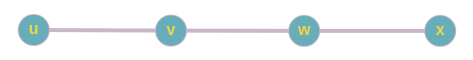
\includegraphics[width=.78\textwidth]{Rysunki/l9z2a.png}}}$ \\
    $\vcenter{\hbox{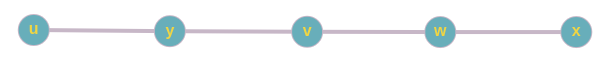
\includegraphics[width=1\textwidth]{Rysunki/l9z2b.png}}}$
\end{figure}

\noindent Na powyższym rysunku wierzchołki $u, x$ mają stopień $1$, a $v, w$ są
stopnia $2$. Dodajemy nowy wierzchołek $y$ taki, że z krawędzi $\{ u, v \}$
powstają dwie nowe: $\{ u, y \}$ oraz $\{ y, w \}$. Jak widzimy, zmieniła się ilość
krawędzi w grafach $G_1$ oraz $G_2$, jednak liczba liści $t_1$ pozostała taka,
jak na samym początku.

\newpage
\noindent \textbf{Zadanie 3} \newline
Pokaż, że graf $G$ jest drzewem wtedy i tylko wtedy gdy dla dowolnej pary
wierzchołków $u, v \in G$ w $G$ istnieje dokładnie jedna ścieżka je łącząca. \\

% \noindent Z definicji graf $G$ jest drzewem wtedy, gdy nie zawiera żadnego cyklu.
% Załóżmy nie wprost, że między wierzchołkami $u, v$ istnieją dwie ścieżki. Weźmy 
% wierzchołki $x, y$ połączone krawędzią i pokażmy, że $\{ x, y \}$ nie jest mostem.

\noindent Mamy udowodnić poniższą tożsamość:
\[  
    G \text{ jest drzewem } \Longleftrightarrow 
    \text{ jest tylko jedna ścieżka pomiędzy } u, v \text{ w } G
\]

\noindent Załóżmy, że $G$ jest spójny, bo gdyby nie był, to $G$ nie byłoby drzewem.
Aby udowodnić twierdzenie z zadania. Przeprowadźmy więc dowód implikacji w obie strony:
\begin{itemize}
    \item [$\Longrightarrow$:] Z definicji wiemy, że aby $G$ było drzewem, to
    w grafie $G$ nie może istnieć żaden cykl, a więc więcej niż jedna ścieżka
    pomiędzy wierzchołkami $u, v$. $\checkmark$
    \item [$\Longleftarrow$:] Weźmy dowolny graf $G$, w którym jest tylko jedna
    ścieżka między wierzchołkami $u, v$. Dołożenie jakiejkolwiek krawędzi do tego
    grafu (bez dodawania nowych wierzchołków) sprawiłoby, że w grafie $G$ powstałby
    jakiś cykl, co byłoby sprzeczne z definicją drzewa, która mówi o tym, że w drzewie
    dla $n$ wierzchołków jest dokładnie $n-1$ krawędzi, przez co $G$ nie byłoby już 
    drzewem. 

    Weźmy drzewo $T$ o wierzchołkach $u, v$ i dołóżmy do niego dwa kolejne wierzchołki
    $x, y$, a następnie utwórzmy krawędzie $\{ u, x \}$ i $\{ v, y \}$. Po takich
    operacjach drzewo $T$ będzie wyglądać nastepująco: 
    \begin{figure}[H]
        \centering
        $\vcenter{\hbox{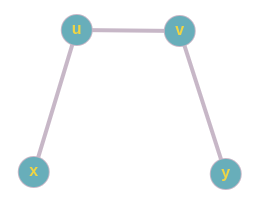
\includegraphics[width=.4\textwidth]{Rysunki/l9z3a.png}}}$
    \end{figure}

    \noindent Jak widzimy, dla $n$ wierzchołków mamy $n-1$ krawędzi. Dołóżmy teraz
    do drzewa $T$ dowolną krawędź, może być to np. $\{ x, y \}$ (lecz dla innych
    krawędzi utworzonych na tym drzewie też będzie to widoczne). Nowy graf wygląda tak:
    \begin{figure}[H]
        \centering
        $\vcenter{\hbox{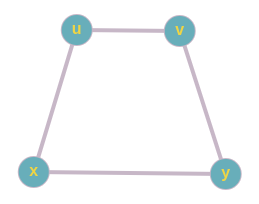
\includegraphics[width=.4\textwidth]{Rysunki/l9z3b.png}}}$
    \end{figure}

    \noindent Jak widać, dodana krawędź tworzy w drzewie cykl, a więc drzewo $T$
    przestaje być drzewem.
\end{itemize}

\noindent Udowodniliśmy więc, że graf $G$ jest drzewem wtedy i tylko wtedy, gdy między
dowolnymi wierzchołkami istnieje tylko jedna ścieżka.

\newpage
\noindent \textbf{Zadanie 5} \newline
Niech $d = \left( d_1, d_2, \ldots, d_n \right)$ będzie ciągiem liczb naturalnych
większych od zera. Wykaż, że $d$ jest ciągiem stopni wierzchołków pewnego drzewa
o $n$ wierzchołkach wtedy i tylko wtedy, gdy $\sum\limits_{i=1}^{n} d_i = 2(n-1)$. \\

\noindent Aby udowodnić powyższe twierdzenie, przeprowadzę dowód w dwie strony:
\begin{itemize}
    \item [$\Longrightarrow$:] Drzewo o $n$ wierzchołkach ma $n-1$ krawędzi, a więc
    z lematu o uściskach dłoni mamy: 
    \[ \sum\limits_{i=1}^{n} d_i = 2 \abs{E} =  2(n-1) \]
    \item [$\Longleftarrow$:] Załóżmy bez straty ogólności, że ciąg stopni jest 
    posortowany malejąco, a więc $d_1 \geq d_2 \geq \ldots \geq d_n$, wtedy dwa
    ostatnie wyrazy będą stopnia $1$, gdyż są liściami. Udowodnię indukcyjnie po
    $n$, że wzór z twierdzenia zachodzi dla wszystkich $n \in \mathbb{N}_+$:
    \begin{enumerate}
        \item Podstawa indukcji: $n = 2$, wtedy $d_1 + d_2 = 2$, a wiedząc, że
        wszystkie wyrazy ciągu $d$ są dodatnie, mamy $d_1 = d_2 = 1$, czyli jest
        to krawędź pomiędzy dwoma wierzchołkami (liściami). $\checkmark$
        \item Krok indukcyjny: załóżmy, że dla $n$ zachodzi 
        $\sum\limits_{i=1}^{n} d_i = 2(n-1)$ i pokażmy, że dla $n+1$ prawdziwe
        jest $\sum\limits_{i=1}^{n+1} d_i = 2\left((n+1)-1 \right) = 2n$. Dodajmy
        teraz nowy wierzchołek $v_{n+1}$ o stopniu $d_{n+1} = 1$. Niech będzie on
        połączony z dowolnym wierzchołkiem $v_j$ (o stopniu $d_j$). Otrzymamy wtedy
        następujący ciąg stopni wierzchołków:
        \[ d_1, d_2, d_3, \ldots, d_j^\prime, \ldots, d_n, d_{n+1} \]
        Skoro nowy wierzchołek jest połączony z $v_j$, to stopień wierzchołka $v_j$
        w nowym ciągu stopni to $d_j^\prime = d_j + 1$. Zsumujmy więc wszystkie
        stopnie wierzchołków po dodaniu $v_{n+1}$:
        \[ 
            \sum\limits_{\substack{i=1 \\i \neq j}}^{n} d_i + d_j^\prime + d_{n+1} 
            = \sum\limits_{i=1}^{n} d_i + 1 + d_{n+1}
            = 2(n-1) + 1 + 1 = 2n 
        \]
        a to chcieliśmy pokazać. $\checkmark$
    \end{enumerate}
\end{itemize}
Udowodniliśmy implikacje w obie strony, a więc twierdzenie jest prawdziwe.

\newpage
\noindent \textbf{Zadanie 6} \newline
Niech $Q_k$ oznacza graf $k$-wymiarowej kostki, tzn. zbiór wierzchołków tego grafu
tworzą wszystkie $k$-elementowe ciągi zer i jedynek, i dwa wierzchołki są sąsiednie
wtedy i tylko wtedy, gdy odpowiadające im ciągi różnią się dokładnie jedną 
współrzędną. Wykaż, że jest to graf dwudzielny. \\

\noindent Aby graf był dwudzielny, musi mieć dwie rozłączne części $V_1, V_2$ takie, 
że $V_1 \cap V_2 = \emptyset$ oraz $V_1 \cup V_2 = V(G)$. Zgodnie z definicją grafu 
$Q_k$ mamy, że krawędzie incydentne są wtedy i tylko wtedy, gdy ich współrzędne 
różnią się tylko o jedną współrzędną. Podzielmy więc zbiór wszystkich wierzchołków
na dwie części: $V_1$, czyli wierzchołki o parzystej liczbie $1$ oraz $V_2$, czyli
wierzchołki o nieparzystej liczbie $1$. Wtedy niemożliwe jest, aby wierzchołki 
z $V_1$ były swoimi sąsiadami, podobnie w przypadku $V_2$ - gdyby były, to wtedy 
wierzchołki z każdej części różniłyby się o więcej niż jedną współrzędną, więc 
taki graf nie byłby grafem $Q_k$. Oznacza to więc, że graf $Q_k$ jest dwudzielny,
co kończy dowód.

\begin{figure}[H]
	\centering
	$\vcenter{\hbox{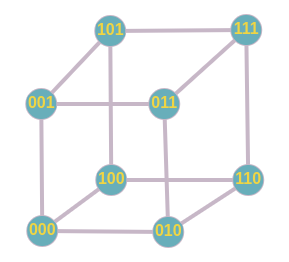
\includegraphics[width=.45\textwidth]{Rysunki/l9z6a.png}}}$
    $\vcenter{\hbox{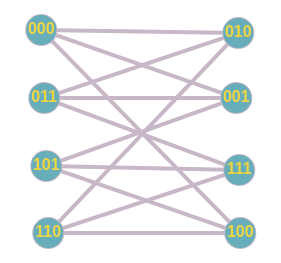
\includegraphics[width=.45\textwidth]{Rysunki/l9z6b.png}}}$
    \\ Przykład: Po lewej stronie przedstawiony został graf $Q_3$ w łatwy sposób
    do narysowania, a po prawej ten sam graf podzielony na rozłączne części $V_1$
    oraz $V_2$. Widać, że wierzchołki o takiej samej parzystości nie są ze sobą
    połączone.
\end{figure}


\newpage
\noindent \textbf{Zadanie 9} \newline
Wykaż, że przynajmniej jeden z grafów $G = (V, E)$ i $\comp{G}$ ($\comp{G}$ jest 
dopełnieniem grafu $G$) jest spójny. Dopełnienie $\comp{G} = (V, E^\prime)$ grafu
$G$ zdefiniowane jest jako graf $(V, E^\prime)$ taki, że $\{ u, v \} \in E^\prime
\Leftrightarrow \{ u, v \} \notin E^\prime$. \\

\noindent Rozpatrzmy dwa przypadki:
\begin{enumerate}
    \item Graf $G$ jest spójny, wtedy przynajmniej jeden z grafów $G$ oraz 
    $\comp{G}$ jest spójny, co kończy ten przypadek, gdyż spełnia założenie
    z zadania.
    \item Graf $G$ nie jest spójny, wtedy jego wierzchołki tworzą co najmniej dwie
    spójne składowe. Weźmy $u, v \in V$. 
    
    Jeśli $u, v \in V$ leżą w dwóch różnych spójnych składowych grafu $G$, więc 
    nie istnieje między nimi krawędź, czyli $\{ u, v \} \notin E$, ale z definicji 
    dopełnienia grafu dostajemy, że $\{ u, v \} \in E^\prime$.

    Niech $u, v \in V$ leżą teraz w jednej spójnej składowej $V_1$ grafu $G$, wtedy
    zgodnie z założeniem, że wierzchołki $G$ tworzą co najmniej dwie spójne składowe 
    wiemy, że istnieje inna (niepusta) spójna składowa $V_2$ taka, że 
    $V_1 \cap V_2 = \emptyset$. Weźmy więc wierzchołek $w \in V_2$, wtedy w grafie
    $G$ nie jest on sąsiadem ani wierzchołka $u$, ani $v$. Oznacza to, że nie
    istnieją krawędzie $\{ u, w \}, \{ v, w \}$ w grafie $G$, a więc muszą one 
    istnieć w $\comp{G}$:
    \[ \{ u, w \}, \{ v, w \} \notin E \Rightarrow \{ u, w \}, \{ v, w \} \in E^\prime \]
    Skoro istnieją takie krawędzie w dopełnieniu, to istnieje ścieżka między 
    wierzchołkami $u$ i $v$ w $\comp{G}$, która przebiega przez wierzchołek $w$
    (czyli $u \to w \to v$).
\end{enumerate}
Udowodniliśmy, że przynajmniej jeden z grafów $G$ i $\comp{G}$ jest spójny.

\end{document}